% !TEX program = xelatex
% AY2013 材料力学 解答例（同志社 生命医科学 医工学コース 院試）
% 問題・図は 01_exams/2013/tex を土台に、参考/ の粒度で解答を付した。
\documentclass[11pt,a4paper]{article}
\usepackage{../../00_common/preamble}
\usetikzlibrary{positioning,arrows.meta,calc,patterns,decorations.pathmorphing}

\title{材料力学 AY2013 解答例（専門応用科目I）}
\author{}
\date{}

\begin{document}
\maketitle

\noindent\textbf{符号規約}：反力・たわみは上向きを正，集中荷重 $P$ は下向き．
モーメントは反時計回りを正とする．せん断力 $Q$ は断面左側に働く上向き外力の和，
曲げモーメント $M$ は下に凸（さがり，上面引張）を正とし，
たわみの基礎式は $EI\,\dfrac{d^2v}{dx^2}=M(x)$ を用いる．
軸力・応力は引張を正とする．

%====================================================================
\section*{〔I〕}

図に示すように片持ちはりの中央 B 点に集中荷重 $P$ が, 右端 C 点に
集中荷重 $P$ と曲げモーメント $M_0\ (=5PL)$ が負荷される問いに答えよ.
はりの縦弾性係数を $E$, 断面形状は幅 $b$, 高さ $h$ の長方形とする.

\begin{center}
\begin{tikzpicture}[>=Latex]
  \draw[thick] (0,0) -- (6,0);
  \draw[thick] (0,-1.0) -- (0,1.0);
  \foreach \y in {-0.9,-0.6,...,0.95} {\draw (0,\y) -- (-0.28,\y+0.28);}
  \node at (0,-0.95) {A};
  \node at (3,-0.35) {B};
  \node at (6,-0.4) {C};
  \draw[->,very thick] (3,1.3) -- (3,0.05) node[midway,left]{$P$};
  \draw[->,very thick] (6,1.7) -- (6,0.05) node[above]{$P$};
  \draw[->,thick] (6.35,0.55) arc (60:-60:0.55) node[midway,right]{$M_0$};
  \draw[<->] (0,1.45) -- (6,1.45) node[midway,fill=white]{$L$};
  \draw[<->] (0,-0.7) -- (3,-0.7) node[midway,fill=white]{$\dfrac{L}{2}$};
  \draw[->] (0,-1.1) -- (1.3,-1.1) node[right]{$x$};
\end{tikzpicture}
\end{center}

\begin{enumerate}[label=(\arabic*)]
  \item 支持点 A に生じる支持力および支持モーメントを図示し,
        つり合い式によりそれらを求めよ.
  \item せん断力 $Q(x)$ と曲げモーメント $M(x)$ を求め,
        せん断力図（SFD）と曲げモーメント図（BMD）を示せ.
  \item 中央 B 点での, はり上面におけるモールの応力円を図示し,
        最大せん断応力を求めよ.
  \item たわみ $v(x)$ に関するはりの基礎式を示し, 積分により
        たわみ角 $\dd v/\dd x=\theta(x)$ とたわみ $v(x)$ を求め,
        C 点におけるたわみ角およびたわみを求めよ.
\end{enumerate}

\subsection*{解答}

\noindent\textbf{(1)}\quad 固定端 A に上向き反力 $R_A$ と反力モーメント $M_A$（反時計回り正）が生じる．
鉛直方向のつり合いより
\[
  R_A - P - P = 0 \;\Longrightarrow\; R_A = 2P.
\]
点 A まわりのモーメントのつり合い（反時計回り正，$M_0$ は時計回りなので $-5PL$）より
\[
  M_A - P\cdot\frac{L}{2} - P\cdot L - 5PL = 0
  \;\Longrightarrow\; M_A = \frac{13}{2}PL.
\]
\[
  \ans{\,R_A = 2P\ (\text{上向き}),\qquad M_A = \frac{13}{2}PL\ (\text{反時計回り})\,}
\]
検算：固定端反力の鉛直成分 $R_A=2P$ は全外力 $P+P=2P$ とつり合う ✓．

\medskip
\noindent\textbf{(2)}\quad 断面左側のつり合いを区間ごとにとる．
$Q$ は左側の上向き外力の和，$M$ は左側外力による曲げ（さがり正）である．

\noindent(I)\ $0\le x<L/2$（区間 AB）：
\[
  Q(x) = R_A = 2P, \qquad M(x) = R_A x - M_A = 2Px - \frac{13}{2}PL.
\]
(II)\ $L/2\le x<L$（区間 BC）：B 点の荷重 $P$ を加えて
\[
  Q(x) = R_A - P = P, \qquad
  M(x) = 2Px - \frac{13}{2}PL - P\!\left(x-\frac{L}{2}\right) = Px - 6PL.
\]
端点・接続点の値：$M(0)=-\dfrac{13}{2}PL$，$M(L/2)=-\dfrac{11}{2}PL$（両式一致），
$M(L^-)=-5PL$．右端 C では $M_0=5PL$ が加わり $-5PL+5PL=0$ となって自由端で 0 ✓．
\[
  \ans{\,Q(x)=\begin{cases}2P & (0\le x<L/2)\\ P & (L/2\le x<L)\end{cases}
  \qquad
  M(x)=\begin{cases}2Px-\dfrac{13}{2}PL & (0\le x<L/2)\\[2mm] Px-6PL & (L/2\le x<L)\end{cases}\,}
\]

\begin{center}
\begin{tikzpicture}[>=Latex,scale=1.0]
  \def\L{2.6}
  \begin{scope}
    \draw[->] (-0.3,0) -- (2*\L+0.6,0) node[right]{$x$};
    \draw[->] (0,-0.3) -- (0,1.6) node[above]{SFD};
    \draw[line width=1pt,blue] (0,1.3) -- (\L,1.3) -- (\L,0.65) -- (2*\L,0.65) -- (2*\L,0);
    \node[left] at (0,1.3) {$2P$}; \node[right] at (0.4,0.55) {$P$};
    \node[below] at (\L,0) {$B$}; \node[below] at (2*\L,0) {$C$}; \node[below] at (0,0) {$A$};
  \end{scope}
  \begin{scope}[xshift=8.5cm]
    \draw[->] (-0.3,0) -- (2*\L+0.6,0) node[right]{$x$};
    \draw[->] (0,-1.6) -- (0,0.5) node[above]{BMD};
    \draw[line width=1pt,red] (0,-1.3) -- (\L,-1.1) -- (2*\L,-1.0) -- (2*\L,0);
    \node[left] at (0,-1.3) {$-\tfrac{13}{2}PL$};
    \node[below] at (\L,-1.1) {$-\tfrac{11}{2}PL$};
    \node[right] at (2*\L,-0.6) {$-5PL$};
    \node[above] at (0,0) {$A$}; \node[above] at (\L,0) {$B$}; \node[above] at (2*\L,0.05) {$C$};
  \end{scope}
\end{tikzpicture}
\end{center}
全区間で $M<0$（上面引張・はりは上に凸の片持ち変形）であり，固定端 A で $|M|$ 最大 $=\dfrac{13}{2}PL$．

\medskip
\noindent\textbf{(3)}\quad B 点（$x=L/2$）の曲げモーメントは $M_B=-\dfrac{11}{2}PL$（大きさ $\dfrac{11}{2}PL$）．
長方形断面の断面二次モーメントは $I=\dfrac{bh^3}{12}$ である．
上面（$y=h/2$）の曲げ応力は，$M_B<0$ より引張で
\[
  \sigma_x = \frac{|M_B|\,(h/2)}{I}
  = \frac{\frac{11}{2}PL\cdot \frac{h}{2}}{bh^3/12}
  = \frac{33PL}{bh^2}.
\]
上面は自由表面かつ曲げの最外縁であるから，せん断応力は $\tau_{xy}=0$，また $\sigma_y=0$．
すなわち単軸応力状態 $(\sigma_x,\ \sigma_y,\ \tau_{xy})=\bigl(\tfrac{33PL}{bh^2},\,0,\,0\bigr)$ である．
モールの応力円は，中心 $\bigl(\tfrac{\sigma_x}{2},0\bigr)$，半径 $\dfrac{\sigma_x}{2}$ の円となる．

\begin{center}
\begin{tikzpicture}[>=Latex,scale=1.0]
  \draw[->] (-0.5,0) -- (4.2,0) node[right]{$\sigma$};
  \draw[->] (0,-1.7) -- (0,1.7) node[above]{$\tau$};
  \draw[line width=1pt,blue] (1.6,0) circle (1.6);
  \fill (3.2,0) circle (0.05) node[below right]{$\sigma_x$};
  \fill (0,0) circle (0.05) node[below left]{$0$};
  \fill (1.6,1.6) circle (0.05) node[above right]{$\tau_{\max}$};
  \draw[dashed] (1.6,0) -- (1.6,1.6);
  \node[below] at (1.6,-0.05) {$\tfrac{\sigma_x}{2}$};
\end{tikzpicture}
\end{center}

最大せん断応力は円の半径に等しく
\[
  \tau_{\max} = \frac{\sigma_x}{2} = \frac{33PL}{2bh^2}.
\]
\[
  \ans{\;\sigma_x=\frac{33PL}{bh^2}\ (\text{引張}),\qquad \tau_{\max}=\frac{33PL}{2bh^2}\;}
\]
検算：単軸応力 $\sigma_x$ のみの状態では主応力は $\sigma_1=\sigma_x,\ \sigma_2=0$ で，
$\tau_{\max}=\dfrac{\sigma_1-\sigma_2}{2}=\dfrac{\sigma_x}{2}$ となり上式と一致する ✓．

\medskip
\noindent\textbf{(4)}\quad たわみの基礎式 $EI\,v''=M(x)$ を各区間で2回積分する．
固定端の境界条件は $v(0)=0,\ v'(0)=0$．

\noindent{}区間 AB（$0\le x\le L/2$）：
\[
  EI\,v_1' = Px^2 - \frac{13}{2}PL\,x,\qquad
  EI\,v_1 = \frac{P}{3}x^3 - \frac{13}{4}PL\,x^2
\]
（$v'(0)=v(0)=0$ より積分定数は 0）．

\noindent{}区間 BC（$L/2\le x\le L$）：
\[
  EI\,v_2' = \frac{P}{2}x^2 - 6PL\,x + C_3,\qquad
  EI\,v_2 = \frac{P}{6}x^3 - 3PL\,x^2 + C_3 x + C_4.
\]
接続条件 $v_1'(L/2)=v_2'(L/2),\ v_1(L/2)=v_2(L/2)$ より
\[
  C_3 = -\frac{PL^2}{8},\qquad C_4 = \frac{PL^3}{48}.
\]
よってたわみ角・たわみは
\[
  \ans{\;EI\,v_1 = \frac{P}{3}x^3 - \frac{13}{4}PL\,x^2,\qquad
        EI\,v_2 = \frac{P}{6}x^3 - 3PL\,x^2 - \frac{PL^2}{8}x + \frac{PL^3}{48}\;}
\]
C 点（$x=L$）でのたわみ角とたわみは
\[
  EI\,\theta_C = EI\,v_2'(L) = \frac{P}{2}L^2 - 6PL^2 - \frac{PL^2}{8} = -\frac{45}{8}PL^2,
\]
\[
  EI\,v_C = EI\,v_2(L) = \frac{P}{6}L^3 - 3PL^3 - \frac{PL^3}{8} + \frac{PL^3}{48} = -\frac{47}{16}PL^3.
\]
\[
  \ans{\;\theta_C = -\frac{45PL^2}{8EI},\qquad
        v_C = -\frac{47PL^3}{16EI}\ \ (\text{下向きに } \tfrac{47PL^3}{16EI})\;}
\]
検算：重ね合わせで確認する．片持ち先端のたわみは，$x=L/2$ の荷重 $P$ で
$\dfrac{5PL^3}{48EI}$，先端 $x=L$ の荷重 $P$ で $\dfrac{PL^3}{3EI}$，
先端モーメント $M_0=5PL$ で $\dfrac{M_0L^2}{2EI}=\dfrac{5PL^3}{2EI}$（いずれも下向き）．
和は $\dfrac{PL^3}{EI}\!\left(\dfrac{5}{48}+\dfrac{16}{48}+\dfrac{120}{48}\right)=\dfrac{47PL^3}{16EI}$ となり一致する ✓．

%====================================================================
\clearpage
\section*{〔II〕}

図に示すように円管（外径 $8d$, 内径 $6d$, 縦弾性係数 $E$）と
テーパ棒（壁面直径 $2d$, 剛体板側直径 $d$, 縦弾性係数 $2E$）からなる
組合せ棒が壁と剛体板に固定されているとき, 次の問い (1) および (2) に答えよ.
ただし, 組合せ棒の自重は無視する. 添字 1 は円管, 添字 2 はテーパ棒を示す.

\begin{center}
\begin{tikzpicture}[>=Latex]
  \draw[thick] (0,-2.2) -- (0,2.2);
  \foreach \y in {-2.1,-1.8,...,2.15} {\draw (0,\y) -- (-0.28,\y+0.28);}
  \draw[line width=2pt] (6,-2.2) -- (6,2.2);
  \fill[pattern=north east lines] (0,1.5) rectangle (6,2.0);
  \fill[pattern=north east lines] (0,-2.0) rectangle (6,-1.5);
  \draw (0,1.5) -- (6,1.5); \draw (0,2.0) -- (6,2.0);
  \draw (0,-1.5) -- (6,-1.5); \draw (0,-2.0) -- (6,-2.0);
  \draw[thick] (0,0.5) -- (6,0.25) -- (6,-0.25) -- (0,-0.5) -- cycle;
  \draw[->,very thick] (6,0) -- (7.4,0) node[right]{$P$};
  \draw[<->] (0,2.35) -- (6,2.35) node[midway,fill=white]{$L$};
  \draw[<->] (0.7,-0.5) -- (0.7,0.5) node[midway,fill=white,font=\scriptsize]{直径 $2d$};
  \draw[<->] (5.3,-0.25) -- (5.3,0.25) node[midway,fill=white,font=\scriptsize]{直径 $d$};
  \draw[->] (0,-2.45) -- (1.3,-2.45) node[right]{$x$};
  \node[align=left] at (1.3,1.0) {\footnotesize テーパ棒\\ \footnotesize $2E,\ \alpha$};
  \node[align=left,anchor=west] at (3.4,2.75) {\footnotesize 円管 外径 $8d$, 内径 $6d$, $E,\ 2\alpha$};
\end{tikzpicture}
\end{center}

\begin{enumerate}[label=(\arabic*)]
  \item 右端の剛体板に外力 $P$ を加えた場合, 内力 $N_1,N_2$, 応力 $\sigma_1(x),\sigma_2(x)$,
        $\sigma_2(x)$ の最大値 $\sigma_{2\max}$, 変位 $\lambda$ を求めよ.
  \item 外力 $P$ を除き, 温度を $\Delta T$ だけ上昇させた.
        このとき内力 $N_{T1}$, $N_{T2}$, 熱応力 $\sigma_{T1}(x)$, $\sigma_{T2}(x)$,
        その最大値 $\sigma_{T2\max}$, および変位 $\lambda_T$ を求めよ.
        熱膨張係数は円管 $2\alpha$, テーパ棒 $\alpha$ とする.
\end{enumerate}

\subsection*{解答}

\noindent\textbf{準備（断面積）}\quad 円管は一様で
\[
  A_1=\frac{\pi}{4}\!\left[(8d)^2-(6d)^2\right]=\frac{\pi}{4}(64-36)d^2=7\pi d^2 .
\]
テーパ棒の直径は壁面（$x=0$）で $2d$，剛体板側（$x=L$）で $d$ と線形変化し
$D_2(x)=d\!\left(2-\dfrac{x}{L}\right)$．したがって
\[
  A_2(x)=\frac{\pi}{4}D_2(x)^2=\frac{\pi}{4}d^2\!\left(2-\frac{x}{L}\right)^{\!2}.
\]
両材は壁と剛体板の間に\textbf{並列}に固定され，剛体板が動くので両材の伸びは等しい（適合条件）．
なお後の積分で用いる量は
\[
  \int_0^L \frac{dx}{A_2(x)}=\frac{4}{\pi d^2}\int_0^L\frac{dx}{(2-x/L)^2}
  =\frac{4}{\pi d^2}\cdot\frac{L}{2}=\frac{2L}{\pi d^2}.
\]

\medskip
\noindent\textbf{(1)}\quad 外力 $P$ は剛体板を介して両材に分配される．自由体（剛体板）の
力のつり合いより，両材はともに引張で
\[
  N_1 + N_2 = P. \tag{つり合い}
\]
両材とも軸力一定．伸びを等置する適合条件は
\[
  \lambda=\frac{N_1 L}{E A_1}
  =\frac{N_2}{2E}\int_0^L\frac{dx}{A_2(x)}
  =\frac{N_2}{2E}\cdot\frac{2L}{\pi d^2}=\frac{N_2 L}{E\pi d^2}.
\]
$A_1=7\pi d^2$ を代入すると $\dfrac{N_1}{7}=N_2$，すなわち $N_1=7N_2$．
つり合い式と連立して
\[
  \ans{\;N_1=\frac{7}{8}P,\qquad N_2=\frac{1}{8}P\;}
\]
応力は
\[
  \sigma_1=\frac{N_1}{A_1}=\frac{7P/8}{7\pi d^2}=\frac{P}{8\pi d^2},\qquad
  \sigma_2(x)=\frac{N_2}{A_2(x)}=\frac{P}{2\pi d^2\left(2-\dfrac{x}{L}\right)^{2}}.
\]
$\sigma_2$ は断面積最小の剛体板側 $x=L$ で最大．
\[
  \ans{\;\sigma_1=\frac{P}{8\pi d^2},\quad
  \sigma_2(x)=\frac{P}{2\pi d^2\left(2-\frac{x}{L}\right)^{2}},\quad
  \sigma_{2\max}=\sigma_2(L)=\frac{P}{2\pi d^2}\;}
\]
変位は
\[
  \ans{\;\lambda=\frac{N_1 L}{EA_1}=\frac{(7P/8)L}{E\cdot 7\pi d^2}=\frac{PL}{8E\pi d^2}\;}
\]
検算：テーパ棒側から $\dfrac{N_2 L}{E\pi d^2}=\dfrac{(P/8)L}{E\pi d^2}=\dfrac{PL}{8E\pi d^2}$ となり，
円管側の $\lambda$ と一致する ✓．

\medskip
\noindent\textbf{(2)}\quad 外力を除き温度を $\Delta T$ 上昇させる．外力がないので自由体のつり合いより
\[
  N_{T1}+N_{T2}=0 .
\]
円管（膨張係数 $2\alpha$）はテーパ棒（$\alpha$）より大きく伸びたいが，並列拘束により
円管は圧縮，テーパ棒は引張となる．伸び（熱＋弾性）を等置する適合条件は
\[
  \lambda_T = 2\alpha\,\Delta T\,L + \frac{N_{T1}L}{EA_1}
            = \alpha\,\Delta T\,L + \frac{N_{T2}}{2E}\cdot\frac{2L}{\pi d^2}.
\]
$N_{T2}=-N_{T1}$，$A_1=7\pi d^2$ を代入して整理すると
\[
  \frac{N_{T1}}{7\pi d^2}+\frac{N_{T1}}{\pi d^2}=-E\alpha\,\Delta T
  \;\Longrightarrow\;
  \frac{8}{7}\frac{N_{T1}}{\pi d^2}=-E\alpha\,\Delta T .
\]
ゆえに
\[
  \ans{\;N_{T1}=-\frac{7}{8}\pi E\alpha\,\Delta T\,d^2\ (\text{圧縮}),\qquad
        N_{T2}=+\frac{7}{8}\pi E\alpha\,\Delta T\,d^2\ (\text{引張})\;}
\]
熱応力は
\[
  \sigma_{T1}=\frac{N_{T1}}{A_1}=\frac{-\frac{7}{8}\pi E\alpha\Delta T d^2}{7\pi d^2}
  =-\frac{E\alpha\,\Delta T}{8},
\]
\[
  \sigma_{T2}(x)=\frac{N_{T2}}{A_2(x)}
  =\frac{\frac{7}{8}\pi E\alpha\Delta T d^2}{\frac{\pi}{4}d^2(2-x/L)^2}
  =\frac{7E\alpha\,\Delta T}{2\left(2-\dfrac{x}{L}\right)^{2}}.
\]
\[
  \ans{\;\sigma_{T1}=-\frac{E\alpha\Delta T}{8},\quad
  \sigma_{T2}(x)=\frac{7E\alpha\Delta T}{2\left(2-\frac{x}{L}\right)^{2}},\quad
  \sigma_{T2\max}=\sigma_{T2}(L)=\frac{7E\alpha\,\Delta T}{2}\;}
\]
変位は円管側から
\[
  \lambda_T = 2\alpha\Delta T L + \frac{N_{T1}L}{EA_1}
  = 2\alpha\Delta T L - \frac{1}{8}\alpha\Delta T L = \frac{15}{8}\alpha\,\Delta T\,L .
\]
\[
  \ans{\;\lambda_T=\frac{15}{8}\alpha\,\Delta T\,L\;}
\]
検算：テーパ棒側から $\alpha\Delta T L+\dfrac{N_{T2}L}{E\pi d^2}
=\alpha\Delta T L+\dfrac{7}{8}\alpha\Delta T L=\dfrac{15}{8}\alpha\Delta T L$ となり，
円管側の $\lambda_T$ と一致する ✓．また $N_{T1}+N_{T2}=0$ で力もつり合う ✓．

\end{document}
